\heading{固体物理学-15春-期末}
\noteinfo{题面依据原始 Word 文档精修录入；原件中的结构图与能带图按物理含义作示意复刻；现有解答为依据题面整理并重新推导的参考答案。}

\begin{question}[16 分]
单层 $\mathrm{MoS_2}$ 有图示的两种配位结构，其中实心圆表示 Mo 原子，空心圆表示 S 原子。
\begin{center}
\begin{tikzpicture}[scale=0.84]
  \begin{scope}[xshift=0cm]
    \node at (0.15,2.15) {A：$1H$-$\mathrm{MX_2}$};
    \coordinate (T1) at (-0.95,0.82); \coordinate (T2) at (0.95,0.82); \coordinate (T3) at (0,-0.88);
    \coordinate (D1) at (-0.67,0.28); \coordinate (D2) at (1.23,0.28); \coordinate (D3) at (0.28,-1.42);
    \coordinate (M1) at (0.14,-0.30);
    \draw[densely dashed] (T1)--(T2)--(T3)--cycle;
    \draw[densely dashed] (D1)--(D2)--(D3)--cycle;
    \draw[densely dashed] (T1)--(D1) (T2)--(D2) (T3)--(D3);
    \fill (M1) circle (4pt);
    \node[anchor=west] at (0.36,-0.22) {$M$};
    \foreach \p in {T1,T2,T3,D1,D2,D3}{
      \draw[thick] (M1)--(\p); \draw[thick,fill=white] (\p) circle (3.4pt);
    }
    \node at (-1.48,1.18) {$X_1$}; \draw[->] (-1.28,1.10)--(-1.00,0.88);
    \node at (-1.48,-0.52) {$X_2$}; \draw[->] (-1.27,-0.45)--(-0.72,0.20);
    \draw[->,thick] (1.70,-1.30)--(1.70,1.42) node[above] {$z$};
    \node at (0.15,-1.92) {三棱柱配位};
  \end{scope}
  \draw[gray] (3.25,-1.80)--(3.25,2.10);
  \begin{scope}[xshift=6.25cm]
    \node at (0,2.15) {B：$1T$-$\mathrm{MX_2}$};
    \coordinate (U1) at (0,1.20); \coordinate (U2) at (-1.04,-0.60); \coordinate (U3) at (1.04,-0.60);
    \coordinate (L1) at (0,-1.20); \coordinate (L2) at (-1.04,0.60); \coordinate (L3) at (1.04,0.60);
    \coordinate (M2) at (0,0);
    \draw[densely dashed] (U1)--(U2)--(U3)--cycle;
    \draw[densely dashed] (L1)--(L2)--(L3)--cycle;
    \fill (M2) circle (4pt); \node[anchor=west] at (0.22,0.08) {$M$};
    \foreach \p in {U1,U2,U3,L1,L2,L3}{
      \draw[thick] (M2)--(\p); \draw[thick,fill=white] (\p) circle (3.4pt);
    }
    \node at (-1.50,1.25) {$X_1$}; \draw[->] (-1.27,1.17)--(-0.10,1.20);
    \node at (-1.50,-1.25) {$X_2$}; \draw[->] (-1.27,-1.17)--(-0.10,-1.20);
    \draw[->,thick] (1.70,-1.30)--(1.70,1.42) node[above] {$z$};
    \node at (0,-1.92) {八面体配位};
  \end{scope}
\end{tikzpicture}
\end{center}
\begin{enumerate}
  \item 两种结构的 $z$ 轴分别是几重旋转轴？（2 分）
  \item 判断两种结构所属的点群并简述理由。可从 $C_3$、$D_{3d}$、$D_{3h}$、$D_{6h}$、$O_h$ 中选择。（4 分）
  \item ZnS 有闪锌矿与纤锌矿两种结构。判断下图 A、B 分别属于哪一种。（2 分）
\end{enumerate}
\begin{center}
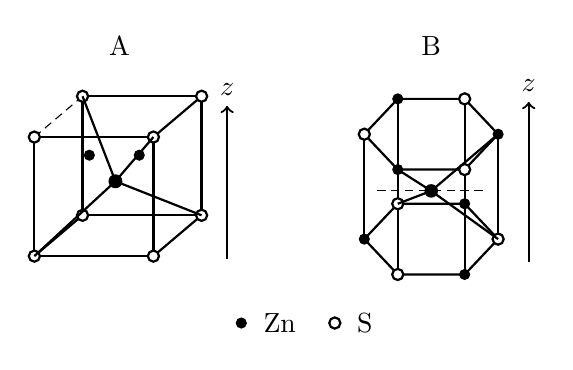
\begin{tikzpicture}[scale=0.72]
  \begin{scope}[xshift=0cm]
    \node at (0.35,2.70) {A};
    \coordinate (f1) at (-1.15,-1.00); \coordinate (f2) at (0.95,-1.00);
    \coordinate (f3) at (0.95,1.10);   \coordinate (f4) at (-1.15,1.10);
    \coordinate (b1) at (-0.30,-0.28); \coordinate (b2) at (1.80,-0.28);
    \coordinate (b3) at (1.80,1.82);   \coordinate (b4) at (-0.30,1.82);
    \draw[thick] (f1)--(f2)--(f3)--(f4)--cycle;
    \draw[thick] (b1)--(b2)--(b3)--(b4)--cycle;
    \draw[thick] (f1)--(b1) (f2)--(b2) (f3)--(b3);
    \draw[densely dashed] (f4)--(b4) (b4)--(b3) (b4)--(b1);
    \foreach \p in {f1,f2,f3,f4,b1,b2,b3,b4}{\draw[thick,fill=white] (\p) circle (2.8pt);}
    \coordinate (ZA) at (0.28,0.32);
    \fill (ZA) circle (3.5pt);
    \draw[thick] (ZA)--(f1) (ZA)--(f3) (ZA)--(b2) (ZA)--(b4);
    \fill (0.70,0.78) circle (2.8pt);
    \fill (-0.18,0.78) circle (2.8pt);
    \draw[->,thick] (2.25,-1.05)--(2.25,1.65) node[above] {$z$};
  \end{scope}
  \begin{scope}[xshift=5.85cm]
    \node at (0,2.70) {B};
    \foreach \a in {0,60,...,300}{
      \coordinate (hb\a) at ({1.18*cos(\a)},{0.72*sin(\a)-0.70});
      \coordinate (ht\a) at ({1.18*cos(\a)},{0.72*sin(\a)+1.15});
    }
    \draw[thick] (hb0)--(hb60)--(hb120)--(hb180)--(hb240)--(hb300)--cycle;
    \draw[thick] (ht0)--(ht60)--(ht120)--(ht180)--(ht240)--(ht300)--cycle;
    \foreach \a in {0,60,...,300}{\draw[thick] (hb\a)--(ht\a);}
    \foreach \a in {0,120,240}{\draw[thick,fill=white] (hb\a) circle (2.8pt); \fill (ht\a) circle (2.8pt);}
    \foreach \a in {60,180,300}{\fill (hb\a) circle (2.8pt); \draw[thick,fill=white] (ht\a) circle (2.8pt);}
    \coordinate (WB) at (0,0.15); \fill (WB) circle (3.4pt);
    \draw[thick] (WB)--(hb0) (WB)--(hb120) (WB)--(ht240) (WB)--(ht0);
    \draw[densely dashed] (-0.95,0.15)--(0.95,0.15);
    \draw[->,thick] (1.72,-1.10)--(1.72,1.72) node[above] {$z$};
  \end{scope}
  \fill (2.50,-2.18) circle (2.8pt); \node[anchor=west] at (2.72,-2.18) {Zn};
  \draw[thick,fill=white] (4.15,-2.18) circle (2.8pt); \node[anchor=west] at (4.37,-2.18) {S};
\end{tikzpicture}
\end{center}
继续回答：
\begin{enumerate}
  \setcounter{enumi}{3}
  \item 对 A 结构，分别判断绕 $z$ 轴转动 $\pi/2$、转动 $\pi$，以及转动 $\pi/2$ 后再作空间反演，晶体是否与原结构重合。（6 分）
  \item B 结构绕 $z$ 轴至少转动多少角度与原结构重合？（2 分）
\end{enumerate}


\begin{solution}
\begin{enumerate}
  \item A 的上下两层 S 原子为三棱柱配位，绕 $z$ 轴转动 $120^\circ$ 重合，故主轴为三重轴；转动 $60^\circ$ 会交换不等价的局域位置，不能单独重合。B 的八面体配位同样具有三重主轴。因此
  \[
    \boxed{A:C_3,\qquad B:C_3.}
  \]
  \item $1H$ 结构有 $C_3$ 主轴、三个面内二重轴和水平镜面 $\sigma_h$，但无反演中心，故
  \[
    \boxed{A:D_{3h}.}
  \]
  $1T$ 结构有 $C_3$ 主轴、三个二重轴和反演中心，上、下 S 层经反演互换，故
  \[
    \boxed{B:D_{3d}.}
  \]
  \item A 为立方单胞，表示\textbf{闪锌矿}结构；B 为六方单胞，表示\textbf{纤锌矿}结构。
  \item 闪锌矿的 Bravais 格子为 FCC，但两套子晶格沿 $(a/4,a/4,a/4)$ 错开。绕 $[001]$ 轴作 $C_4$ 会把基元变到不等价位置，所以转动 $\pi/2$ 后\textbf{不重合}；$C_2=C_4^2$ 是对称操作，转动 $\pi$ 后\textbf{重合}。晶体具有四重反轴 $\bar4=IC_4$，故转动 $\pi/2$ 后再反演\textbf{重合}：
  \[
    \boxed{C_4:\text{否},\quad C_2:\text{是},\quad IC_4:\text{是}.}
  \]
  \item 纤锌矿沿 $c$ 轴具有六重螺旋/宏观点群六重对称。若允许晶体空间群中伴随的平移，最小转角为
  \[
    \boxed{60^\circ=\pi/3.}
  \]
  若只考察不带平移的局域点群操作，则应根据原题给出的具体基元区分 $C_6$ 与 $C_3$；图示通常意在前者。
\end{enumerate}
\end{solution}
\end{question}

\begin{question}[12 分]
V 族元素砷与锑可形成类似石墨烯的起伏蜂窝结构。下图给出结构与能带的示意。
\begin{center}
\begin{tikzpicture}[scale=0.70]
  % Structural panel, following the original plan-view lattice and enlarged side view.
  \begin{scope}[xshift=-0.25cm]
    \node at (2.15,3.35) {砷烯/锑烯起伏蜂窝结构};
    \node[anchor=east] at (-0.15,1.30) {俯视};
    \foreach \m in {0,...,3}{
      \foreach \n in {0,...,1}{
        \pgfmathsetmacro{\ax}{1.18*\m+0.59*\n}
        \pgfmathsetmacro{\ay}{1.02*\n+0.72}
        \coordinate (PA\m\n) at (\ax,\ay);
        \coordinate (PB\m\n) at (\ax,\ay+0.68);
        \draw[thick] (PA\m\n)--(PB\m\n);
        \ifnum\n>0
          \draw[thick] (PA\m\n)--({\ax-0.59},{\ay-0.34});
          \draw[thick] (PA\m\n)--({\ax+0.59},{\ay-0.34});
        \fi
      }
    }
    \foreach \m in {0,...,3}{\foreach \n in {0,...,1}{
      \draw[thick,fill=white] (PA\m\n) circle (2.7pt);
      \fill (PB\m\n) circle (2.7pt);
    }}
    \draw[densely dashed,very thick]
      (PA00)--(PA10)--(PA11)--(PA01)--cycle;

    \node[anchor=east] at (-0.15,-0.25) {侧视};
    \foreach \i in {0,...,5}{
      \pgfmathsetmacro{\xx}{0.78*\i}
      \pgfmathsetmacro{\yy}{-0.55+0.48*mod(\i,2)}
      \ifodd\i
        \fill (\xx,\yy) circle (3pt);
      \else
        \draw[thick,fill=white] (\xx,\yy) circle (3pt);
      \fi
      \ifnum\i<5
        \pgfmathsetmacro{\xn}{0.78*(\i+1)}
        \pgfmathsetmacro{\yn}{-0.55+0.48*mod(\i+1,2)}
        \draw[thick] (\xx,\yy)--(\xn,\yn);
      \fi
    }
    \draw[<->,thick] (4.18,-0.55)--(4.18,-0.07)
      node[midway,right=2pt] {$d=1.35\,\text{\AA}$};
  \end{scope}

  % Multi-band sketch of the original As-monolayer band plot.
  \begin{scope}[xshift=6.55cm,yshift=-0.05cm]
    \node at (2.30,3.72) {As monolayer};
    \draw[->] (-0.12,0)--(4.90,0);
    \draw[->] (0,-0.12)--(0,3.55) node[above] {$E$};
    \foreach \x/\lab in {0/$\Gamma$,1.75/$M$,2.95/$K$,4.55/$\Gamma$}{
      \draw[densely dashed] (\x,0)--(\x,3.38);
      \node[below=2pt] at (\x,0) {\lab};
    }
    % Conduction bands.
    \draw[thick] plot[smooth] coordinates {(0,2.48) (0.55,2.68) (1.25,2.55) (1.75,2.62) (2.35,2.80) (2.95,2.68) (3.70,2.82) (4.55,2.58)};
    \draw[thick] plot[smooth] coordinates {(0,2.72) (0.60,2.98) (1.20,2.84) (1.75,2.96) (2.35,2.83) (2.95,3.12) (3.75,3.02) (4.55,2.91)};
    \draw[thick] plot[smooth] coordinates {(0,2.92) (0.55,3.16) (1.20,3.10) (1.75,3.24) (2.35,3.05) (2.95,3.28) (3.70,3.18) (4.55,3.25)};
    \draw[thick] plot[smooth] coordinates {(0,3.18) (0.55,3.30) (1.30,3.22) (1.75,3.34) (2.45,3.18) (2.95,3.36) (3.70,3.28) (4.55,3.34)};
    % Valence bands.
    \draw[thick] plot[smooth] coordinates {(0,1.60) (0.60,1.54) (1.20,1.38) (1.75,1.48) (2.35,1.42) (2.95,1.52) (3.70,1.46) (4.55,1.62)};
    \draw[thick] plot[smooth] coordinates {(0,1.40) (0.55,1.22) (1.20,1.30) (1.75,1.20) (2.35,1.08) (2.95,1.20) (3.70,1.15) (4.55,1.30)};
    \draw[thick] plot[smooth] coordinates {(0,1.12) (0.60,0.94) (1.20,1.04) (1.75,0.92) (2.35,0.86) (2.95,0.98) (3.70,0.90) (4.55,1.05)};
    \draw[thick] plot[smooth] coordinates {(0,0.48) (0.70,0.28) (1.35,0.22) (1.75,0.40) (2.35,0.62) (2.95,0.72) (3.70,0.52) (4.55,0.30)};
    \draw[thick] plot[smooth] coordinates {(0,0.16) (0.60,0.30) (1.25,0.52) (1.75,0.60) (2.35,0.50) (2.95,0.30) (3.70,0.18) (4.55,0.36)};
    \draw[<->,thick] (0.62,1.62)--(0.62,2.45);
    \node[anchor=west] at (0.78,2.04) {$\Delta=2.49\,\mathrm{eV}$};
  \end{scope}
\end{tikzpicture}
\end{center}
\begin{enumerate}
  \item 从价电子数目的角度说明砷与锑为何可形成蜂窝状结构。（4 分）
  \item 画出该结构的布拉伐格子，并指出其特征。（2 分）
  \item 砷烯能隙约为 $2.49\,\mathrm{eV}$。根据能带图判断它是否适合作为发光材料，并说明理由。（2 分）
  \item 单层 $\mathrm{MoS_2}$ 的最低光学吸收能量约为 $1.8\,\mathrm{eV}$。仅据此断言砷烯的能隙一定大于 $\mathrm{MoS_2}$ 是否可靠？说明理由。（4 分）
\end{enumerate}


\begin{solution}
\begin{enumerate}
  \item As、Sb 均有 5 个价电子。起伏蜂窝中每个原子与三个近邻形成三条 $\sigma$ 共价键，消耗三个电子；余下两个电子形成一个孤对。其局域构型接近 $sp^3$ 杂化，因此平面结构容易起伏以降低键角应变。这与 C 的四价、平面 $sp^2$ 蜂窝不同。
  \item 蜂窝点阵不是 Bravais 格子，而是\textbf{二维三角 Bravais 格子加两个原子基元}。原胞含 A、B 两个等价（无外场时）子晶格原子，维格纳--塞茨胞为正六边形。
  \item 从图中可见价带最高点与导带最低点出现在不同 $k$ 点，即为\textbf{间接带隙}。电子--空穴辐射复合还需声子提供准动量，几率显著小于直接跃迁。因此仅从该图判断，砷烯不如直接带隙材料适合作高效率发光材料。
  \item 不可靠。最低光学吸收峰对应的是光学激发能
  \[
    E_{\rm opt}=E_g^{\rm qp}-E_B^{\rm exciton},
  \]
  其中 $E_g^{\rm qp}$ 是准粒子带隙，$E_B^{\rm exciton}$ 是激子结合能。二维材料屏蔽弱，激子结合能可很大；此外间接带隙、缺陷态和声子辅助吸收也会影响吸收边。因此 $1.8\,\mathrm{eV}$ 不能直接等同于 MoS$_2$ 的单粒子带隙，不能据此严格比较二者带隙。
\end{enumerate}
\end{solution}
\end{question}

\begin{question}[10 分]
\begin{enumerate}
  \item 有人认为：周期绝缘体不导电、无序体系中局域态不导电以及半导体中带电杂质束缚态不导电，三者机制相同。判断该说法并说明理由。（4 分）
  \item 从低能激发的角度比较导体与非导体。（4 分）
  \item 布拉伐格子是否必然具有空间反演对称？实际晶格是否也必然具有空间反演对称？（2 分）
\end{enumerate}


\begin{solution}
\begin{enumerate}
  \item 说法错误。周期绝缘体的本征态通常是延展 Bloch 态，不导电是因为价带全满且与空导带之间有能隙；无序体系的局域态因相干多重散射在实空间指数局域，费米能处即使有态也不能扩散；带电杂质束缚态则由局域 Coulomb 势形成氢型离散能级，载流子需热电离或场电离后才能进入延展带。三者分别是能隙、无序局域化和局域势束缚机制。
  \item 导体在热力学极限中具有任意低能的带电激发：费米面附近有占据态和空态，施加弱场即可使分布发生偏移。普通绝缘体或半导体的最低带电激发需跨越有限能隙 $E_g$；局域化体系虽可能无谱隙，但直流输运的延展激发有迁移率边或局域化障碍。故“是否存在能量趋零且能携带电流的延展激发”是关键。
  \item 任意 Bravais 格子若含格点 $\vb R$，也必含 $-\vb R$，因为整数系数可同时变号，所以它总有以格点为中心的反演对称。实际晶格还含基元；反演后基元若不能借助平移与自身重合，则晶体无反演中心。故
  \[
    \boxed{\text{Bravais 格子必有反演；实际晶格未必有}.}
  \]
\end{enumerate}
\end{solution}
\end{question}

\begin{question}[10 分]
考虑周期为 $a$ 的一维周期势，在近自由电子近似下回答：
\begin{enumerate}
  \item 为什么布里渊区边界会打开能隙？（2 分）
  \item 在布里渊区边界，电子群速度、准动量 $\hbar\vb k$ 以及动量算符平均值分别是多少？（6 分）
  \item 能带波函数 $\psi_{n\vb k}(\vb r)$ 是否总可写成平面波与周期函数之积？是否总可写成布洛赫和
  \[
  \psi_{n\vb k}(\vb r)=\frac1{\sqrt N}\sum_l
  \ee^{\ii\vb k\cdot\vb R_l}W_n(\vb r-\vb R_l),
  \]
  其中 $W_n$ 为空间局域函数？（2 分）
\end{enumerate}


\begin{solution}
\begin{enumerate}
  \item 在区边界 $k=G/2=\pi/a$，自由电子态 $\ket{k}$ 与 $\ket{k-G}$ 具有相同能量。周期势的 Fourier 分量 $V_G$ 把它们耦合，简并微扰矩阵
  \[
    \begin{pmatrix}E_0&V_G\\V_G^*&E_0\end{pmatrix}
  \]
  的本征值为 $E_0\pm\abs{V_G}$，故打开
  \[
    \boxed{E_g=2\abs{V_G}}
  \]
  的能隙。对应波函数为两行波的驻波组合，在离子附近概率密度不同，势能期望值因而不同。
  \item 区边界是能带极值，故
  \[
    \boxed{v_g=\frac1\hbar\frac{\dd E}{\dd k}=0.}
  \]
  准动量仍为
  \[
    \boxed{\hbar k=\pm\frac{\pi\hbar}{a}}
  \]
  且两者模 $\hbar G$ 等价。区边界驻波含等权的 $+\pi/a$ 与 $-\pi/a$ 平面波分量；对局域势哈密顿量
  $\langle p\rangle=m\langle v\rangle=m v_g$，所以
  \[
    \boxed{\langle p\rangle=0.}
  \]
  这正说明准动量不等于真实动量平均值。
  \item 对任意周期单电子哈密顿量，Bloch 定理保证
  \[
    \boxed{\psi_{n\vb k}=\ee^{\ii\vb k\cdot\vb r}u_{n\vb k},
    \quad u_{n\vb k}(\vb r+\vb R)=u_{n\vb k}(\vb r).}
  \]
  对一个孤立且拓扑平庸的能带，可由 Bloch 态 Fourier 变换构造局域 Wannier 函数，并反写成题给 Bloch 和。普通一维无磁场能带满足这一条件。更一般地，具有非零 Chern 数的单带不能选取全局光滑规范，从而不存在同时指数局域且保持全部要求的单带 Wannier 函数；此时需把若干能带组成复合带处理。
\end{enumerate}
\end{solution}
\end{question}

\begin{question}[12 分]
价带顶部的 $\vb k$ 态缺失一个电子，该电子在 $\vb k$ 处的有效质量为 $m_e^*$。
\begin{enumerate}
  \item 求整个价带产生的电流 $\vb I$，并求外加电磁场 $(\vb E,\vb B)$ 下电流的变化率 $\dd\vb I/\dd t$，给出证明。（10 分）
  \item 某界面附近价带向上弯曲，空穴由右向左运动。对该空穴而言，这段能带弯曲对应势垒还是势阱？说明理由。（2 分）
\end{enumerate}
\begin{center}
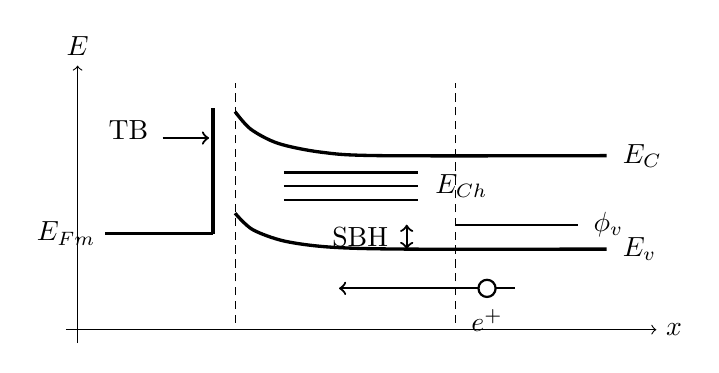
\begin{tikzpicture}[x=1cm,y=0.86cm]
  \draw[->] (-0.15,0)--(7.35,0) node[right] {$x$};
  \draw[->] (0,-0.20)--(0,3.90) node[above] {$E$};
  \draw[densely dashed] (2.00,0.10)--(2.00,3.65);
  \draw[densely dashed] (4.80,0.10)--(4.80,3.65);

  % Metal Fermi level and the interface barrier (TB).
  \draw[thick] (0.35,1.42)--(1.72,1.42);
  \node[anchor=east] at (0.35,1.42) {$E_{Fm}$};
  \draw[very thick] (1.72,1.42)--(1.72,3.28);
  \node[anchor=east] at (1.02,2.95) {TB};
  \draw[->,thick] (1.08,2.83)--(1.67,2.83);

  % Semiconductor conduction band and interface-localized levels.
  \draw[very thick] plot[smooth] coordinates
    {(2.00,3.22) (2.20,2.96) (2.55,2.75) (3.10,2.62) (3.85,2.57) (6.72,2.57)};
  \node[anchor=west] at (6.80,2.57) {$E_C$};
  \foreach \yy in {2.32,2.12,1.92}{
    \draw[thick] (2.62,\yy)--(4.32,\yy);
  }
  \node[anchor=west] at (4.42,2.12) {$E_{Ch}$};

  % Valence band, tail level, hole barrier and hole motion.
  \draw[very thick] plot[smooth] coordinates
    {(2.00,1.72) (2.22,1.48) (2.62,1.31) (3.20,1.22) (4.15,1.19) (6.72,1.19)};
  \node[anchor=west] at (6.80,1.19) {$E_v$};
  \draw[thick] (4.80,1.55)--(6.35,1.55);
  \node[anchor=west] at (6.43,1.55) {$\phi_v$};
  \draw[<->,thick] (4.18,1.19)--(4.18,1.55)
    node[midway,left=3pt] {SBH};
  \draw[<-,thick] (3.32,0.61)--(5.55,0.61);
  \draw[thick,fill=white] (5.20,0.61) circle (3.1pt);
  \node[below=4pt] at (5.20,0.61) {$e^+$};
\end{tikzpicture}
\end{center}


\begin{solution}
\begin{enumerate}
  \item 满价带的总电流为零，因为周期性给出
  \[
    \sum_{\vb k\in\mathrm{BZ}}\vb v_v(\vb k)
    =\frac1\hbar\sum_{\vb k}\grad_{\vb k}E_v(\vb k)=0.
  \]
  若缺少一个位于 $\vb k_e$ 的电子，该电子原本贡献
  $\vb j_e=-e\vb v_e(\vb k_e)/V$，故剩余价带电流为其相反数：
  \[
    \boxed{\vb j=\frac eV\vb v_e(\vb k_e).}
  \]
  定义空穴波矢 $\vb k_h=-\vb k_e$、能量
  $E_h(\vb k_h)=E_v^{\max}-E_v(-\vb k_h)$，则
  \[
    \vb v_h=\frac1\hbar\grad_{\vb k_h}E_h
    =\vb v_e(\vb k_e),
  \]
  所以 $\vb j=e\vb v_h/V$，空穴等效带电 $+e$。

  在各向同性抛物近似下
  \[
    \frac1{m_h^*}=-\frac1{m_e^*},
  \]
  因价带顶电子 $m_e^*<0$，故 $m_h^*>0$。空穴半经典运动方程为
  \[
    \hbar\dot{\vb k}_h=e(\vb E+\vb v_h\times\vb B).
  \]
  又 $\dot{\vb v}_h=\hbar\dot{\vb k}_h/m_h^*$，因此单个空穴电流变化率
  \[
    \boxed{\frac{\dd\vb j}{\dd t}
    =\frac{e^2}{Vm_h^*}(\vb E+\vb v_h\times\vb B).}
  \]
  若有空穴密度 $p$，则把 $1/V$ 替换为 $p$。

  \item 空穴势能与价带顶相反，可写为
  $U_h(x)=\text{const}-E_v(x)$。图中 $E_v$ 向右升高，所以 $U_h$ 向右降低。空穴从右向左运动时由低势能区走向高势能区，故该弯曲对它是
  \[
    \boxed{\text{势垒}.}
  \]
\end{enumerate}
\end{solution}
\end{question}

\begin{question}[14 分]
取均匀磁场的对称规范
\[
 \vb A=\frac12(-By,Bx,0),
 \qquad \vb p\longrightarrow\vb p+q\vb A.
\]
\begin{enumerate}
  \item 从哈密顿量的变化说明金属或半导体中载流子的朗道运动使体系能量升高还是降低。（6 分）
  \item 存在外磁场时，哈密顿量的复共轭是否等于自身？体系是否具有时间反演不变性？（2 分）
  \item 计入电子自旋磁矩，画出最低四个朗道能级。取 $\mu_{\mathrm B}=\hbar|q|/(2m_0)$，且 $m^*=m_0$。（2 分）
  \item 金属电子在什么条件下可产生自发磁化？（2 分）
  \item 材料的铁磁性与导电性是否存在必然联系？（2 分）
\end{enumerate}


\begin{solution}
\begin{enumerate}
  \item 对电荷 $q$、有效质量 $m^*$ 的载流子，
  \[
    H=\frac{(\vb p+q\vb A)^2}{2m^*}
    =\frac{p^2}{2m^*}+\frac{qB}{2m^*}L_z
    +\frac{q^2B^2}{8m^*}(x^2+y^2).
  \]
  $A^2$ 项为正，完整对角化得到
  \[
    E_{n,k_z}=\hbar\omega_c\left(n+\frac12\right)
    +\frac{\hbar^2k_z^2}{2m^*},
    \qquad \omega_c=\frac{\abs{qB}}{m^*}.
  \]
  相对于无场连续横向运动，轨道被量子化；每个固定 $n$ 的零点轨道能为正，外场使体系自由能出现正的二阶变化，对应 Landau 抗磁性
  $M=-\partial F/\partial B<0$。
  \item 复共轭把 $\vb p=-\ii\hbar\grad$ 变为 $-\vb p$，因此
  \[
    H(B)^*=H(-B)\ne H(B)
  \]
  （在固定规范下亦可相差规范变换）。时间反演同时反转动量、自旋和外磁场，故有外加固定 $B\ne0$ 时体系不具有时间反演不变性。
  \item 计入自旋 Zeeman 能，取电子 $g=2$、$m^*=m_0$：
  \[
    E_{n,s}=\hbar\omega_c\left(n+\frac12\right)+s\mu_BB,
    \qquad s=\pm1,
  \]
  且 $\mu_BB=\hbar\omega_c/2$。故
  \[
    E_{n,-}=n\hbar\omega_c,
    \qquad E_{n,+}=(n+1)\hbar\omega_c.
  \]
  最低状态依次为 $0$，$\hbar\omega_c$（二重），$2\hbar\omega_c$（二重）等；忽略轨道简并时最低四个 $(n,s)$ 可列为
  $(0,-),(0,+),(1,-),(1,+)$。
  \item 巡游电子需满足 Stoner 判据
  \[
    \boxed{I D(E_F)>1,}
  \]
  即交换能降低超过把两自旋能带分裂所需的动能代价，顺磁态才对自发自旋极化不稳定。
  \item 无必然联系。Fe、Co、Ni 是导电铁磁体；铁氧体、EuO 等可为绝缘铁磁体；Cu、Ag 等金属又不铁磁。铁磁性由交换相互作用及能态决定，导电性由费米能处是否有延展态决定，两者可相关但不是互为充要条件。
\end{enumerate}
\end{solution}
\end{question}

\begin{question}[16 分]
\begin{enumerate}
  \item 决定电子在不同区域之间净流动方向的物理量是什么？（2 分）
  \item 画出 PNP 结接触前与接触后的空间能带图。（6 分）
  \item 从能带角度说明平衡时该结为何不导通。（2 分）
  \item 应在 P 区施加正门压还是负门压才能使该结导通？画出导通状态的空间能带图。（4 分）
  \item 若不施加门压，但 N 区长度只有数纳米，载流子是否可能通过？说明理由。（2 分）
\end{enumerate}


\begin{solution}
\begin{enumerate}
  \item 决定净流动方向的是\textbf{电化学势}，电子语言中即局域费米能（非平衡时为准费米能）。粒子从较高电化学势流向较低电化学势，直至平衡时 $E_F$ 处处相同。
  \item 对标准 P--N--P 结构，接触前各区能带平直，P 区 $E_F$ 靠近 $E_v$，N 区 $E_F$ 靠近 $E_c$。接触后费米能水平，电子能带在两个 P 区较高、中央 N 区较低，形成两个耗尽层；对空穴而言中央 N 区是势垒。
  \begin{center}
  \begin{tikzpicture}[x=1cm,y=0.82cm]
  \draw[->] (0,0)--(8.25,0) node[right] {$x$};
  \draw[->] (0,-0.35)--(0,4.25) node[above] {$E$};
  \draw[densely dashed] (0.35,2.08)--(7.72,2.08);
  \node[anchor=west] at (7.78,2.08) {$E_F$};
  \draw[densely dashed] (2.45,0.15)--(2.45,3.88);
  \draw[densely dashed] (5.55,0.15)--(5.55,3.88);

  % At equilibrium the two band edges remain parallel and the gap is constant.
  \draw[very thick] plot[smooth] coordinates
    {(0.35,3.18) (1.50,3.18) (2.05,3.02) (2.55,2.55) (3.18,2.24) (4.82,2.24) (5.45,2.55) (5.95,3.02) (6.50,3.18) (7.55,3.18)};
  \draw[very thick] plot[smooth] coordinates
    {(0.35,1.26) (1.50,1.26) (2.05,1.10) (2.55,0.63) (3.18,0.32) (4.82,0.32) (5.45,0.63) (5.95,1.10) (6.50,1.26) (7.55,1.26)};
  \node[anchor=west] at (7.62,3.18) {$E_c$};
  \node[anchor=west] at (7.62,1.26) {$E_v$};
  \node at (1.28,3.72) {P};
  \node at (4.00,3.72) {N};
  \node at (6.72,3.72) {P};

  % Hole barrier measured from the P-region valence-band edge to the N-region edge.
  \draw[densely dotted] (1.52,1.26)--(4.34,1.26);
  \draw[<->,thick] (4.34,0.32)--(4.34,1.26)
    node[midway,right=3pt] {$\Delta E_h$};
  \node at (4.00,-0.22) {中央 N 区为空穴势垒};
\end{tikzpicture}
  \end{center}
  \item 平衡时 $E_F$ 水平，扩散流与内建电场造成的漂移流相互抵消；中央区对多数载流子形成有限势垒，且没有外加电化学势差，所以净电流为零。
  \item 门压的符号必须结合“门加在哪一区”和“希望输运哪种载流子”说明。正门压提高静电势 $\phi$，使电子能带整体下移 $\Delta E=-e\Delta\phi$；负门压使能带上移。标准 P--N--P 以空穴导通时，应使中央 N 区的 $E_v$ 上移、空穴势垒降低，因此对中央 N 区加\textbf{负门压}。若回忆版原意是 N--P--N 且门加在中央 P 区、以电子导通，则应加\textbf{正门压}使中央 $E_c$ 下移。题面“PNP”与“在 P 区加门压”不足以唯一确定几何，判据是
  \[
    \boxed{\text{把多数载流子所见的中央势垒压低}.}
  \]
  \item 即使无门压，当势垒宽度只有数纳米时，载流子波函数可穿透耗尽区。WKB 透射率约为
  \[
    T\sim\exp\left[-2\int\frac{\sqrt{2m^*(U-E)}}\hbar\,\dd x\right],
  \]
  宽度越小指数抑制越弱，因此可能出现隧穿电流；高温下还可有热激发越过势垒。
\end{enumerate}
\end{solution}
\end{question}

\begin{question}[10 分]
把晶体势写成原子势之和，以 $\vb R_n$ 为中心的原子势为 $V(\vb r-\vb R_n)$，原子偏离平衡位置的位移为 $\vb u_n$。
\begin{enumerate}
  \item 当所有原子均发生小位移时，写出晶格势能的一阶变化。（2 分）
  \item 波矢为 $\vb q$、振幅为 $A$、偏振方向为 $\vb e$ 的声子，使布洛赫电子由 $\vb k$ 跃迁至 $\vb k'$，其矩阵元为
  \[
  \left\langle\vb k'\left|
  \sum_n\frac A2\ee^{\pm\ii\vb q\cdot\vb R_n}
  \vb e\cdot\grad V(\vb r-\vb R_n)
  \right|\vb k\right\rangle.
  \]
  证明该矩阵元必然给出晶体准动量守恒。（6 分）
  \item 为什么碳纳米管等刚性较强的材料中，电子通常具有较长的弛豫时间？（2 分）
\end{enumerate}


\begin{solution}
\begin{enumerate}
  \item 原子位移后
  $V(\vb r-\vb R_n-\vb u_n)$ 作 Taylor 展开：
  \[
    V(\vb r-\vb R_n-\vb u_n)
    \simeq V(\vb r-\vb R_n)
    -\vb u_n\cdot\grad V(\vb r-\vb R_n).
  \]
  因此晶格势的一阶变化为
  \[
    \boxed{\delta V(\vb r)=-\sum_n\vb u_n\cdot
    \grad V(\vb r-\vb R_n).}
  \]
  题给矩阵元若把位移相位或 $A$ 的符号吸收进定义，整体负号不影响选择定则。
  \item 对 Bloch 态使用平移性质。把积分按原胞分块并令
  $\vb r=\boldsymbol\rho+\vb R_n$，则每一项除相位外相同：
  \[
  \begin{aligned}
  M_{\vb k'\vb k}^{\pm}
  &\propto\sum_n\ee^{\pm\ii\vb q\cdot\vb R_n}
  \int_{\rm cell}\dd^3\rho\,
  \psi_{\vb k'}^*(\boldsymbol\rho+\vb R_n)
  \vb e\cdot\grad V(\boldsymbol\rho)
  \psi_{\vb k}(\boldsymbol\rho+\vb R_n)\\
  &\propto\sum_n\ee^{\ii(\vb k-\vb k'\pm\vb q)\cdot\vb R_n}M_{\rm cell}.
  \end{aligned}
  \]
  晶格和满足
  \[
    \sum_n\ee^{\ii\vb Q\cdot\vb R_n}
    =N\sum_{\vb G}\delta_{\vb Q,\vb G}.
  \]
  因此矩阵元非零必须有
  \[
    \boxed{\vb k'=\vb k\pm\vb q-\vb G}
  \]
  （等价地写成 $\vb k\pm\vb q=\vb k'+\vb G$），即电子与声子过程的晶体准动量模倒格矢守恒。
  \item 刚性强意味着键的力常数大、声子频率高。给定量子数下原子零点或热位移振幅
  \[
    u_{\vb q s}\propto\sqrt{\frac{\hbar}{M\omega_{\vb q s}}}
  \]
  较小，晶格势的一阶扰动以及低频声子的热占据也较小，电子--声子散射率降低，故弛豫时间通常较长。碳材料的高声速还减小了低能声子态密度。
\end{enumerate}
\end{solution}
\end{question}
